% !TEX root = ../oddp.tex

\section{The Milnor resolution and the periodic resolution}\label{s:milnor_to_per}
In this section we will construct a map $\chains(\partial\asimplex^{r-1})^{\ot n+1}\to \Per{r}$ that intertwines $\theta_j$ and $\theta$ (\cref{prop:milnor_to_per}), with $r$ an odd number.
This construction depends on building a \emph{weak codegeneracy}, something that is attained in \cref{prop:construction_xi}. Finally, in \cref{prop:straightenings} we will show that each $r$-cyclic straightening with duality yields a weak codegeneracy.  

\subsection{From the Milnor resolution to the periodic resolution} Let $\sigma = [0,1,\ldots,r-1]$ denote the positively oriented top generator of $\asimplex^{r-1}$, with $r$ an odd number. There is a chain map $h\colon \sus{r-1}\chains(\asimplex^{r-1})\to \chains(\asimplex^{r-1})$ that sends every generator to zero except for $h([v]) = \sigma$ if $[v]$ has degree $1$ and $h(\varnothing) = \partial \sigma$. %I understand that $[v]$ has deg 1 before suspension, but maybe should be written differently.
\begin{definition}
	The \emph{augmented periodic resolution of $\Cyc_r$} is the graded $R$-module $\Per{r} = \chains(\partial\asimplex^{r-1})\oplus \bigoplus_{m>0} \sus{(r-1)m} \chains(\partial \simplex^{r-1})$ with the following differential: if $[v]$ is an element of degree $1$, then
	\[
		\partial(\sus{(r-1)m}[v]) = \sus{(r-1)(m-1)}h\circ \partial([v]) = \sus{(r-1)(m-1)}\partial\circ h([v]),
	\]
	on other degrees, we take the differential of the tensor product. %What tensor product?
\end{definition}
Define the \emph{periodicity map} $\theta \colon \sus{r-1}\Per{r}\to \Per{r}$ as %Aren''t there too many \thetas already?
\[
	\theta(\sus{(r-1)m}\tau) = \sus{(r-1)(m+1)}\tau
\]
in degrees $>0$ and by $\theta(\varnothing) = \partial \sigma$. Recall the maps $$\theta_0,\theta_1\colon \chains(\partial\asimplex^{r-1})\to \chains(\partial\asimplex^{r-1})^{\ot 2}$$ given by
\begin{align*}
	\theta_0(\tau) &= \partial \sigma \ot \rho^{-1}(\tau) 
	&
	\theta_1(\tau) &= \tau \ot \partial \sigma
\end{align*}

%\begin{definition}
	%We write $\chains(\asimplex^{r-1})^{\text{per}}$ for the chain complex $\chains(\partial\simplex^{r-1})$ considered with $\bZ_r$-grading and the usual differential, except that $\partial([v]) = \partial \sigma$.
%\end{definition}

\begin{definition}\label{def:weak_codegeneracy}
	A $\Cyc_r$-equivariant chain map $\xi\colon \chains(\partial\asimplex^{r-1})^{\otimes 2}\to \Per{r}$ is a \emph{weak codegeneracy} if:
	\begin{enumerate}
		\item $\xi(\tau_1\otimes \tau_2) = \tau_1*\tau_2$ if $|\tau_1| + |\tau_2| \leq r-1$,
		\item $(\xi\circ \theta_0)(\tau) = \theta(\tau)$,
		\item $(\xi\circ \theta_1)(\tau) = \theta(\tau)$.
	\end{enumerate}
\end{definition}

\begin{proposition}\label{prop:milnor_to_per}
	A weak codegeneracy $\xi$ induces a chain map 
	\[
		\psi\colon \chains(\partial \asimplex^{r-1})^{\otimes (n+1)}\to \Per{r}
	\]
	defined recursively on $n$ as:
	\begin{align*}
		\psi(\tau) &= \tau & \text{if $n=0$}, \\
		\psi(\tau_0\ot \tau_1 \ldots \ot \tau_n) &=  \psi(\tau_0\otimes \ldots\otimes \xi(\tau_{n-1}\otimes \tau_n)) &\text{if $n>0$.} %& \text{if $|\tau_{n-1}| + |\tau_n| < r$} \\
%			\psi(\tau_0\otimes \ldots \otimes  \tau_n) &= \sus{(r-1)} \psi(\tau_0\otimes \ldots\otimes  \xi(\tau_{n-1}\otimes \tau_n)) & \text{if $|\tau_{n-1}| + |\tau_n| \geq r$}
	\end{align*}
	In addition, $\psi\circ \theta_j = \theta\circ \psi$ for each $j=0\ldots n$.
\end{proposition} %No proof? 


\subsection{Barycentric subdivisions}\label{s:assembly}

Recall that the barycentric subdivision $\sd \partial\simplex^{r-1}$ of the boundary of the standard simplex $\simplex^{r-1}$ is the simplicial complex that has one vertex for each non-empty face of $\simplex^{r-1}$ and one face $(\tau_0,\dots,\tau_k)$ of dimension $k$ for every ascending chain $\tau_0 \subset \tau_1\subset\dots \subset \tau_k$ of simplices of $\partial \simplex^{r-1}$. We will denote the face $(\tau_0 \subset \dots \subset \tau_k)$ as $[\bar{\tau}_0|\bar{\tau}_1|\dots|\bar{\tau}_k]$, where $\bar{\tau}_i = \tau_i\smallsetminus \tau_{i-1}$ is the face such that the geometric join $\bar{\tau}_i\star \tau_{i-1}$ is the face $\tau_i$. With this notation, the differential on $\chains(\sd \partial \simplex^{r-1})$ becomes
\[
\partial([\bar{\tau}_0|\bar{\tau}_1|\dots|\bar{\tau}_k]) = \sum_{i=0}^{k-1} (-1)^i[\bar{\tau}_0|\dots|\bar{\tau}_i\star \bar{\tau}_{i+1}|\dots |\bar{\tau}_k] + (-1)^k [\bar{\tau}_0|\dots|\bar{\tau}_{k-1}].
\]

The \emph{pair barycentric subdivision} $\Psd \partial\simplex^{r-1}$ of $\partial \simplex^{r-1}$ is a cubulation of $\partial \simplex^{r-1}$ with the same vertices as $\sd \partial \simplex^{r-1}$ and one face for each pair $(a,b)$ of faces of $\partial\simplex^{r-1}$ such that $b \subset a$ (cf. \cite{Rounds2010}). Geometrically, that face is the union of all the faces of dimension $|a|-|b|$ of the barycentric subdivision that correspond to ascending chains $b = \tau_0 \subset \dots \subset \tau_k= a$. Interpreting $b$ as a dual cochain, its chain complex $\chains(\Psd \partial\simplex^{r-1})$ is isomorphic to the tensor product $\chains(\partial\simplex^{r-1}) \ot \cochains(\partial\simplex^{r-1})$ modulo the pairs $a \ot b$ such that the support of $b$ is not contained in $a$.

These constructions are related by the following chain maps
\[
\xymatrix{
%	&\susp{-n-1}\chains(\partial\simplex^n) \ot \chains(\partial\simplex^n)\ar[d]^h& \\
	\chains(\partial\simplex^{r-1})\ar[r]^{s_*^{\simplex}}\ar@/_2.0pc/[rr]^{s_*} & \susp{}\chains(\Psd \partial\simplex^{r-1})\ar[r]^{s^{\Psd}_*} & \chains(\sd\partial\simplex^{r-1})
}
\]
defined as follows: if $[a_0,\dots,a_{k-1}]\in \chains(\partial\simplex^{r-1})$ is an ordered representative of a generator,
\begin{align*}
	s_*([a_0,\dots,a_{k-1}]) &= \sum_{\perm\in \Sigma_{k}} (-1)^{\sign{\perm}}[a_{\perm(0)}|a_{\perm(1)}|\dots|a_{\perm(k-1)}],
	\\
	s_*^{\simplex}([a_0,\dots,a_{k-1}]) &= (-1)^{k-1}\sum_{j=0}^{k-1} [a_0,\dots,a_{k-1}]\ot (a_j).
\end{align*}
If $b = (b_0,\dots,b_{m-1})\in \cochains(\partial\simplex^{r-1})$ and $a = [c_0,\dots,c_{\ell-1},b_0,\dots,b_{m-1}]\in \chains(\partial\simplex^{r-1})$ with $k = m+\ell$, then
\begin{equation}\label{eq:sP}
	s_*^{\Psd}( a\ot b) = (-1)^{m} \sum_{\perm\in \Sigma_{\ell}} (-1)^{\sign{\perm}} [b|c_{\perm(0)}|c_{\perm(1)}|\dots|c_{\perm(\ell-1)}]
\end{equation}
Notice that the letter $b$ plays a different role in each side: on the left, it is a dual generator of the normalized cochain complex, thus it makes sense to permute its entries changing the generator by a sign. On the right, $b$ is a vertex of $\sd\partial\simplex^{r-1}$.

Consider the following endomorphisms of the chain complexes of the barycentric and the pair subdivision
\begin{align*}
	\alex \colon \chains(\sd \partial\simplex^{r-1})& \lra \chains(\sd \partial\simplex^{r-1}),
	&
	\alex \colon \chains(\Psd \partial\simplex^{r-1})& \lra \chains(\Psd \partial\simplex^{r-1}).
\end{align*}
The first one sends an ascending chain of simplices $\tau_0 \subset \dots \subset \tau_{k-1}$ to the ascending chain of their complementary simplices $(-1)^{\binom{k}{2}} \tau_{k-1}^c \subset \dots\subset\tau_0^c$, which in our notation becomes $[\bar{\tau}_0|\bar{\tau}_1|\dots|\bar{\tau}_{k-1}]\mapsto (-1)^{\binom{k}{2}}[\tau_{k-1}^c|\bar{\tau}_{k-1}|\dots|\bar{\tau}_1]$.
The second one sends $a \ot b$ to $\twist\circ \left(\alex \ot \alex^{-1}\right)(a \ot b)$, where $\twist\colon C\ot D\to D\ot C$ is the chain map $\twist(x\ot y) = (-1)^{|x||y|}y\ot x$. \martin{I would change a bit the notation of this duality maps. Right now it says $\Lambda=\twist\circ(\alex\ot\alex^{-1})$. Maybe $\alex_{P}$ and $\alex_{\sd}$.}
\begin{lemma}\label{lemma:diag_alex_twist} The following diagram commutes.
	\begin{equation*}\label{diag:newdiag}
		\xymatrix{
			\susp{-r}\chains(\partial \simplex^{r-1})\ot \chains(\partial\simplex^{r-1})\ar[r]^-{\id\ot \Lambda}\ar[d]^{\twist} %\ar@{}[dr] | {(-1)^{n+1}}
			&\chains(\Psd \partial \asimplex^{r-1}) \ar[r]^{s_*^{\Psd}}\ar[d]_{\alex} %\ar@{}[dr] | {(-1)^{n+1}}
			& \susp{-1}\chains(\sd \partial \asimplex^{r-1})\ar[d]^{\alex}\\
			\susp{-r}\chains(\partial \simplex^{r-1})\ot \chains(\partial\simplex^{r-1})\ar[r]^-{\id \ot \Lambda} &\chains(\Psd \partial \asimplex^{r-1}) \ar[r]^{s_*^{\Psd}}& \susp{-1}\chains(\sd \partial \asimplex^{r-1}).
		}
	\end{equation*}
\end{lemma}

\begin{proof}
	For the first square, we have
	\begin{align*}
		\twist\circ(\Lambda \ot \Lambda^{-1})\circ (\id\ot \alex)
		&=  \twist\circ(\alex \ot \id)
		=  (\id\ot \alex) \circ \twist.
	\end{align*}
	For the second square, with the notation of \eqref{eq:sP}, let
	$$a\ot b =  [c_0,\dots,c_{\ell-1},b_0,\dots,b_{m-1}]\ot(b_0,\dots,b_{m-1})$$ 
	be a generator of $\chains(\Psd \partial\asimplex^{r-1})$ such that both $b=[b_0,\dots,b_{m-1}]$ and $c=[c_0,\dots,c_{\ell-1}]$ are ordered, and suppose additionally that $a = [a_0,\dots,a_k]$ is the result of ordering $[b_0,\dots,b_{m-1},c_0,\dots,c_{\ell-1}]$. Then,
	\begin{equation}\label{eq:lastsign}
		\begin{split}
			\alex\circ s_*^{\Psd} (a \ot b)                                                        
			&= (-1)^{m}\sum_{\perm} (-1)^{\sign{\perm}} \alex[b|c_{\perm(0)}|\dots|c_{\perm(\ell-1)}]
			\\
			&= (-1)^{m} \sum_{\perm} (-1)^{\sign{\perm}} (-1)^{\binom{\ell+1}{2}} [a^c|c_{\perm(\ell-1)}|\dots|c_{\perm(0)}]
			\\
			&= (-1)^{m}\sum_{\perm'} (-1)^{\sign{\perm'}} (-1)^{\binom{\ell+1}{2}} (-1)^{\binom{\ell}{2}} [a^c|c_{\perm'(0)}|\dots|c_{\perm'(\ell-1)}]
			\\
			&= (-1)^{k}\sum_{\perm'} (-1)^{\sign{\perm'}} [a^c|c_{\perm'(0)}|\dots|c_{\perm'(\ell-1)}]
		\end{split}
	\end{equation}
	(be aware that the penultimate equality equates the summand indexed by a permutation $\perm$ with the summand indexed by the permutation $\perm' = \perm\circ \mathrm{rev}$, where $\mathrm{rev}$ is the permutation that sends $(0,1,\dots,\ell-2,\ell-1)$ to $(\ell-1,\ell-2,\dots,1,0)$. The sign of the permutation $\mathrm{rev}$ is the sign $(-1)^{\binom{\ell}{2}}$.

 Let $x=[x_0,\dots,x_{n-k}]$ be the ordered complement of $a$, and let $y=[y_0,\dots,y_{n-m}]$ be the ordered complement of $b$. Recall that we denote by $\lambda(a,b)$ the sign that orders $a\cup b$. Then $s_*^{\Psd}\circ \Lambda$ produces the following sign:
	\[
	\xymatrix{
		 [c_0,\dots,c_{\ell-1},b_0,\dots,b_{m-1}] \ot (b_0,\dots,b_{m-1})
		\ar[d]^-{(-1)^{\lambda(c,b)}}_-{\sim}
		\\
 [a_0,\dots,a_{k-1}] \ot (b_0,\dots,b_{m-1})
		\ar[d]^{(-1)^{kr+\lambda(a,x)+\lambda(y,b)}}_{\Lambda\ot \Lambda^{-1}}
		\\
	(x_0,\dots,x_{r-k-1}) \ot [y_0,\dots,y_{r-m-1}]
		\ar[d]^-{(-1)^{(r-k)(r-m)}}_-{\twist}
		\\
		[y_0,\dots,y_{r-m-1}] \ot (x_0,\dots,x_{r-k-1})
		\ar[d]^-{(-1)^{\lambda(c,x)}}_-{\sim}
		\\
		[c_0,\dots,c_{\ell-1},x_0,\dots,x_{r-k-1}] \ot (x_0,\dots,x_{r-k-1}) 
		\ar[d]_{s_*^{\Psd}}^{{(-1)}^{r-k}}
		\\
		\sum_{\perm} (-1)^{\sign{\perm}}[x| c_{\perm(0)}|\dots|c_{\perm(\ell-1)}]
	}
	\]
	Now, $\lambda(c,b) + \lambda(a,x)$ computes the sign of the permutation that orders
	\[
	[c_0,\dots,c_{\ell-1},b_0,\dots,b_{m-1},x_{0},\dots,x_{r-k-1}],
	\]
	and $\lambda(c,x) + \lambda(y,b)$ computes the sign of the permutation that orders
		\[
	[c_0,\dots,c_{\ell-1},x_{0},\dots,x_{r-k-1},b_0,\dots,b_{m-1}],
	\]
	thus their sum computes the sign of the permutation that interchanges $x_0,\ldots,x_{r-k-1}$ and $b_0,\ldots,b_{m-1}$, which is $(r-k)m$. Now,
	\[
	(r-k)m + kr + (r-k)(r-m) + (r-k) \equiv k.
	\]
Since the sign of \eqref{eq:lastsign} was $(-1)^{k}$, the second square commutes on the nose.
\end{proof}



\subsection{Constructing a weak codegeneracy and cyclic straightenings}

\begin{definition}
	An \emph{assemblage map} is a simplicial map $g \colon \sd \partial \simplex^{r-1} \to \partial \simplex^{r-1}$ such that the composition of chain maps $g_*\circ s_*$ is the identity.
\end{definition}

\begin{definition}
	An \emph{$r$-cyclic assemblage map} is an assemblage map $g \colon \sd \partial \simplex^{r-1} \to \partial \simplex^{r-1}$ that is cyclic with respect to the forward action of the cyclic group $\Cyc_{r}$.
\end{definition}

\begin{definition}
	An \emph{$r$-cyclic assemblage map with duality} is an $r$-cyclic assemblage map $g$ such that the composition
	\[\sd \partial \simplex^{r-1} \overset{\alex}{\lra} \sd \partial\simplex^{r-1} \overset{g}{\lra} \partial\simplex^{r-1}\overset{\rho^{-1}}{\lra} \partial\simplex^{r-1} \]
	is also an assemblage map.
\end{definition}

\begin{proposition}\label{prop:construction_xi}
	If $g$ is an $r$-cyclic assemblage map with duality, then there is a weak codegeneracy $\xi\colon \chains(\asimplex^{r-1})\ot \chains(\asimplex^{r-1})\to \Per{r}$ given by $\xi(a\ot b) = a*b$ if $|a|+|b|<r$ and by the following composition otherwise: \martin{I would change the places for the suspensions so it matches the target:{\small
	\[
		\chains(\partial \simplex^{r-1})\otimes \chains(\partial \simplex^{r-1})
		\overset{\id\otimes \alex}{\lra}
		\susp{r}\chains(\Psd\partial\simplex^{r-1})
		\overset{s_*^{\Psd}}{\lra}
		\susp{r-1}\chains(\sd\partial\simplex^{r-1})
		\overset{g_*}{\lra}
		\susp{r-1}\chains(\partial\simplex^{r-1}).
	\]
	}}
	{\small
	\[
		\susp{-r}\chains(\partial \simplex^{r-1})\otimes \chains(\partial \simplex^{r-1})
		\overset{\id\otimes \alex}{\lra}
		\chains(\Psd\partial\simplex^{r-1})
		\overset{s_*^{\Psd}}{\lra}
		\susp{-1}\chains(\sd\partial\simplex^{r-1})
		\overset{g_*}{\lra}
		\susp{-1}\chains(\partial\simplex^{r-1}).
	\]
	}
\end{proposition}
\begin{proof} It is clear that the resulting map is equivariant and a chain map in degrees different from $r$. If $a\otimes b \in \chains(\partial\simplex^{r-1})\ot \chains(\partial\simplex^{r-1})$ is an element of degree $r$, we have to check that 
\begin{equation}\label{eq:771}
	\partial\circ \xi(a\otimes b) = \text{join}\circ \partial (a\ot b),
\end{equation}
where $\text{join}$ is the join product. For notational purposes, let us assume that $a$ and $b$ are ordered representatives and that $a$ has degree $k$. Recall that $\star$ denotes the geometric join of simplices. Regarding the right hand-side of \eqref{eq:771}, we have that
\[
	\text{join}\circ \partial(a\ot b) = \partial\circ \text{join}(a\ot b)) = \begin{cases} 0 &\text{if $a\star b\neq  \sigma$} \\ (-1)^{\lambda(a,b)} \partial \sigma & \text{if $a\star b = \sigma$}.\end{cases}
\] 
Regarding the left hand-side of \eqref{eq:771},
\[
	\partial\circ \xi(a\ot b) 
	= \partial\circ g_*\circ s^{\Psd}\circ (\id \ot \alex)(a\otimes b) 
	= (-1)^{k}\partial\circ g_*\circ s^{\Psd}(a\otimes \Lambda(b))%why (-1)^k?
\]
which is zero unless $a\star b = \sigma$, in which case it equals
\[
	(-1)^{k}(-1)^{\lambda(b,a)} \partial\circ g_*\circ s^{\Psd}(a\otimes a^\dd)
	= (-1)^{\lambda(b,a)} \partial\circ g_* (a)
	= (-1)^{\lambda(b,a)}\partial \sigma,
\]
because $g_*([a])$ is some vertex $v$ of $\simplex^{r-1}$, and $\partial(v) = \partial\sigma$ in $\Per{r}$. Additionally, notice that $\lambda(a,b)$ and $\lambda(b,a)$ have the same parity because $r$ is odd.


We now check the three conditions of \cref{def:weak_codegeneracy}. The first condition holds by construction. The third condition holds as well:
\begin{equation}\label{eq:508}
\begin{split}
	\xi\circ \theta_1(\tau) &= \xi(\tau\ot \partial\sigma) \\
	&= \sus{r-1} g_*\circ s^{\Psd} \circ (\id \ot \alex) (\tau\ot \partial \sigma) \\
	&= \sus{r-1}(-1)^{|\tau|} g_*\circ s^{\Psd} (\tau\ot \alex(\partial \sigma)) \\
	&= \sus{r-1}(-1)^{|\tau|-1}\sum_{i\in \tau} g_*\circ s^{\Psd} (\tau\ot (i)) \\
	&= \sus{r-1} g_*\circ s^{\Psd} \circ s^{\Delta} (\tau) \\
	&= \sus{r-1} g_*\circ s_*(\tau) \\
	&= \sus{r-1} \tau
\end{split}
\end{equation}
	And for the second condition:
	\begin{align*}
		\xi\circ \theta_0(\tau) &= \xi(\partial\sigma \ot \rho^{-1}(\tau))
		\\
		&\overset{(1)}= \sus{r-1}g_*\circ s_*^{\Psd}\circ (\id\ot \alex)\circ \rho^{-1}(\partial\sigma \ot \tau)
		\\
		&\overset{(2)}{=} \sus{r-1}\rho^{-1}\circ g_*\circ s_*^{\Psd}\circ (\id\ot \alex)\circ \twist(  \tau \ot \partial\sigma)
		\\
		&\overset{(3)}{=} \sus{r-1}\rho^{-1}\circ g_*\circ \alex\circ s_*^{\Psd}\circ (\id\ot \alex)(\tau \ot \partial\sigma)
		\\
		&\overset{(4)}{=} \sus{r-1}\tau.
	\end{align*}
In $(1)$ we use that $\partial\sigma$ is fixed by the action of $\rho$, in $(2)$, that the maps $g,s_*^{\Psd}$ and $\Lambda$ are equivariant, in $(3)$ we use \cref{lemma:diag_alex_twist}, and in (4) we use that $\rho^{-1}\circ g_*\circ \Lambda$ is also an assemblage map, and thus the chain of equalities of \eqref{eq:508} remains valid after replacing $g_*$ for $\rho^{-1}\circ \Lambda\circ g_*$.
\end{proof}


Observe that $\Cyc_r$ acts freely on the vertices of $\partial \simplex^{r-1}$, but it only acts freely on the vertices of $\partial \sd\simplex^{r-1}$ if $r$ is prime. Therefore $r$-cyclic assemblage maps only exist if $r$ is prime. On the other hand, the following lemma, pointed to us by Martin Palmer, assures the existece of such maps when $r$ is prime. %proposition?



\begin{definition}
	An \emph{$r$-straightening} is a choice, for each non-empty proper subset $\tau$ of $\{0,1,\dots,r-1\}$, of an element $x_\tau\in \tau$. An \emph{$r$-cyclic straightening} is an straightening that is equivariant with respect to the action of the cyclic group $\Cyc_r$. An \emph{$r$-cyclic straightening with duality} is an $r$-cyclic straightening such that the cyclic predecessor of $x_\tau$ is not an element of $\tau$.
\end{definition}

\begin{proposition}\label{prop:straightenings}
	Assemblage maps are in bijection with $r$-straightenings, $r$-cyclic assemblage maps are in bijection with $r$-cyclic straightenings, and $r$-cyclic assemblage maps with duality are in bijection with $r$-cyclic straightenings with duality.
\end{proposition}

\begin{proof}
	If $\tau\mapsto x_{\tau}\in \tau$ is an $r$-straightening, we can define an assemblage map $g$ as
	\[
	g(\tau_0\subset\dots\subset\tau_{k-1}) = [x_{\tau_0},\dots,x_{\tau_{k-1}}]
	\]
%	where $\pi$ is the permutation that orders the values on the right. 
	To check that it is an assemblage map,
	\[
	g_*\circ s_*([a_0,\dots,a_{k-1}]) = g\left(\sum_{\perm} (-1)^{\sign{\perm}} (a_{\perm(0)}|\dots|a_{\perm(k-1)})\right)
	\]
	vanishes in all summands except for the summand $(\omega_0 \subset \omega_1 \subset \dots \subset \omega_{k-1})$ defined as
	\begin{align*}
		\omega_{k-1} &= a
		&
		\omega_{i} &= \omega_{i+1}\smallsetminus \{x_{\omega_{i+1}}\}.
	\end{align*}
	Reciprocally, if $g$ is an assemblage map, then $\tau\mapsto g([\tau])$ is a straightening.
	
	The second assertion is evident. For the last one, if $\tau$ is a face of $\sd \partial \simplex^{r-1}$, then $\rho^{-1}(g(\Lambda(\tau))) = \rho^{-1}(x_{\tau^c})$ is the cyclic predecessor of $x_{\tau^c}$, which does not belong to $\tau^c$, and therefore belongs to $\tau$.
\end{proof}

\subsection{Examples}

\begin{example}
	If $r=3$, the only assemblage map with duality comes from the choice
	\begin{align*}
		[0]&\mapsto 0 & [0,1]&\mapsto [0]
	\end{align*}
\end{example}

\begin{example}\label{example:asymmetries5}
	If $r=5$, there are four assemblage maps with duality corresponding to the following choices:
	\begin{align*}
		[0]&\mapsto 0 & [0,1]&\mapsto 0 & [0,2]&\mapsto 0 & [0,1,2]&\mapsto 0 & [0,1,3] & \mapsto 0 & [0,1,2,3] & \mapsto 0 \\
		[0]&\mapsto 0 & [0,1]&\mapsto 0 & [0,2]&\mapsto 2 & [0,1,2]&\mapsto 0 & [0,1,3] & \mapsto 0 & [0,1,2,3] & \mapsto 0 \\
		[0]&\mapsto 0 & [0,1]&\mapsto 0 & [0,2]&\mapsto 0 & [0,1,2]&\mapsto 0 & [0,1,3] & \mapsto 3 & [0,1,2,3] & \mapsto 0 \\
		[0]&\mapsto 0 & [0,1]&\mapsto 0 & [0,2]&\mapsto 2 & [0,1,2]&\mapsto 0 & [0,1,3] & \mapsto 3 & [0,1,2,3] & \mapsto 0
	\end{align*}
\end{example}

If $r=7$ there are several thousands of assemblage maps with duality.

\begin{figure}
	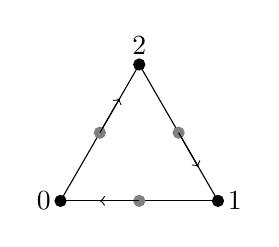
\begin{tikzpicture}
		\draw (0,1.732) -- (1,0);
		\draw (-1,0) -- (1,0);
		\draw (-1,0) -- (0,1.732);
		\filldraw [gray] (-.5,.866) circle (2pt);
		\filldraw [gray] (.5,.866) circle (2pt);
		\filldraw [gray] (0,0) circle (2pt);
		\filldraw [black] (0,1.732) circle (2pt) node[anchor=south]{2};
		\filldraw [black] (1,0) circle (2pt) node[anchor=west]{1};
		\filldraw [black] (-1,0) circle (2pt) node[anchor=east]{0};
		\draw[->] (0,0) -- (-.5,0);
		\draw[->] (-.5,.866) -- (-.25,1.299);
		\draw[->] (.5,.866) -- (.75,.433);
	\end{tikzpicture}
	\caption{The $r$-cyclic assemblage map with duality for $\partial \simplex^2$.}
\end{figure}

\begin{example}\label{example:f3_1}
	For $r=3$, and $a \ot b = [0] \ot [2,1]$ we have:
	\begin{align*}
		\xi([0] \ot [2,1])
		&= g_*\circ s_*^{\Psd}\circ (\id\ot \alex)([0] \ot [2,1])
		\\
		&= -g_*\circ s_*^{\Psd}\circ ([0] \ot \alex([2,1]))
		\\
		&= g_*\circ s_*^{\Psd}([0] \ot (0))
		\\
		&= -g_*([0])
		\\
		&= -[0]
	\end{align*}
	Observe that, since the summand $[1,2]$ appears with positive sign in $\partial \sigma = \partial([0,1,2])$, we have that $\xi([0] \ot \partial\sigma) = [0]$, as dictated by the third condition of \cref{def:weak_codegeneracy}.
\end{example}

\begin{example}\label{example:f3_2}
	For $r=3$ and $a \ot b = [0,1] \ot [2,0]$, we have:
	\begin{align*}
		\xi([0,1] \ot [2,0]) &= g_*\circ s_*^{\Psd}\circ (\id\ot \alex)([0,1] \ot [2,0])
		\\
		&= g_*\circ s_*^{\Psd}([0,1] \ot \alex([2,0]))
		\\
		&= g_*\circ s_*^{\Psd} ([0,1] \ot [1])
		\\
		&= -g_*([1|0])
		\\
		&= -[1,0]
	\end{align*}
	Observe that this exhibits the second and third conditions of \cref{def:weak_codegeneracy}:
	\begin{align*}
		\xi ([0,1] \ot \partial\sigma) &= [0,1]
		&
		\xi(\partial\sigma \ot \rho^{-1}([0,1])) &= [0,1].
	\end{align*}
\end{example}

\begin{example}\label{example:f5_1}
	For $r=5$ and the first $r$-cyclic straightening of Example \ref{example:asymmetries5}, if $a \ot b = [2,3,0] \ot [4,1,3]$, we have:
	\begin{align*}
		\xi([2,3,0] \ot [4,1,3]) &= g_*\circ s_*^{\Psd}\circ (\id\ot \alex)([2,3,0] \ot [4,1,3])
		\\
		&= -g_*\circ s_*^{\Psd}([2,3,0] \ot \Lambda([4,1,3]))
		\\
		&= g_*\circ s_*^{\Psd}([2,3,0] \ot (0,2))
		\\
		&= g_*([02|3])
		\\
		&= [0,2]
	\end{align*}
\end{example}

\begin{example}\label{example:f5_2}
	For $r=5$ and the first $r$-cyclic straightening of Example \ref{example:asymmetries5}, if $a \ot b = [1,2,3,4] \ot [0,1,2]$ we have:
	\begin{align*}
		\xi([1,2,3,4] \ot [0,1,2])
		&= g_*\circ s_*^{\Psd}\circ (\id\ot \alex)([1,2,3,4] \ot [0,1,2])
		\\
		&= g_*\circ s_*^{\Psd}([1,2,3,4] \ot \alex([0,1,2]))
		\\
		&= g_*\circ s_*^{\Psd}([1,2,3,4] \ot [3,4])
		\\
		&= g_*([34|1|2]-[34|2|1])
		\\
		&= [3,3,1] - [3,2,1]
		\\
		&= [1,2,3]
	\end{align*}
	Again, this exhibits the third condition of \cref{def:weak_codegeneracy}: $\xi(\partial\sigma \ot [0,1,2] = [1,2,3])$.
\end{example}


